\documentclass{article}

\usepackage[flushmargin, ragged, side]{footmisc} 

\usepackage[]{amsmath} 
\usepackage[]{xcolor} 
\usepackage[]{amsthm} 
\usepackage[]{amssymb} 
\usepackage[]{enumerate} 
\usepackage[]{graphicx} 
\usepackage[]{subcaption} 
\usepackage[]{hyperref} 
\usepackage[]{cleveref} 

\newcommand{\ua}{\uparrow}
\newcommand{\da}{\downarrow}
\newcommand*{\github}[1]{\def\@github{\color{gray!70}#1}}
\newcommand{\githublogo}{\raisebox{-1pt}{
\includegraphics[height=9pt]{github}}}

\title{%
  \textsc{The Ising model in two dimensions}\\
  \small{FYS3150}
  }
\author{Ivar Haugal\o kken Stangeby}
\begin{document}
  \maketitle
  \begin{figure}[h!]
    \centering
    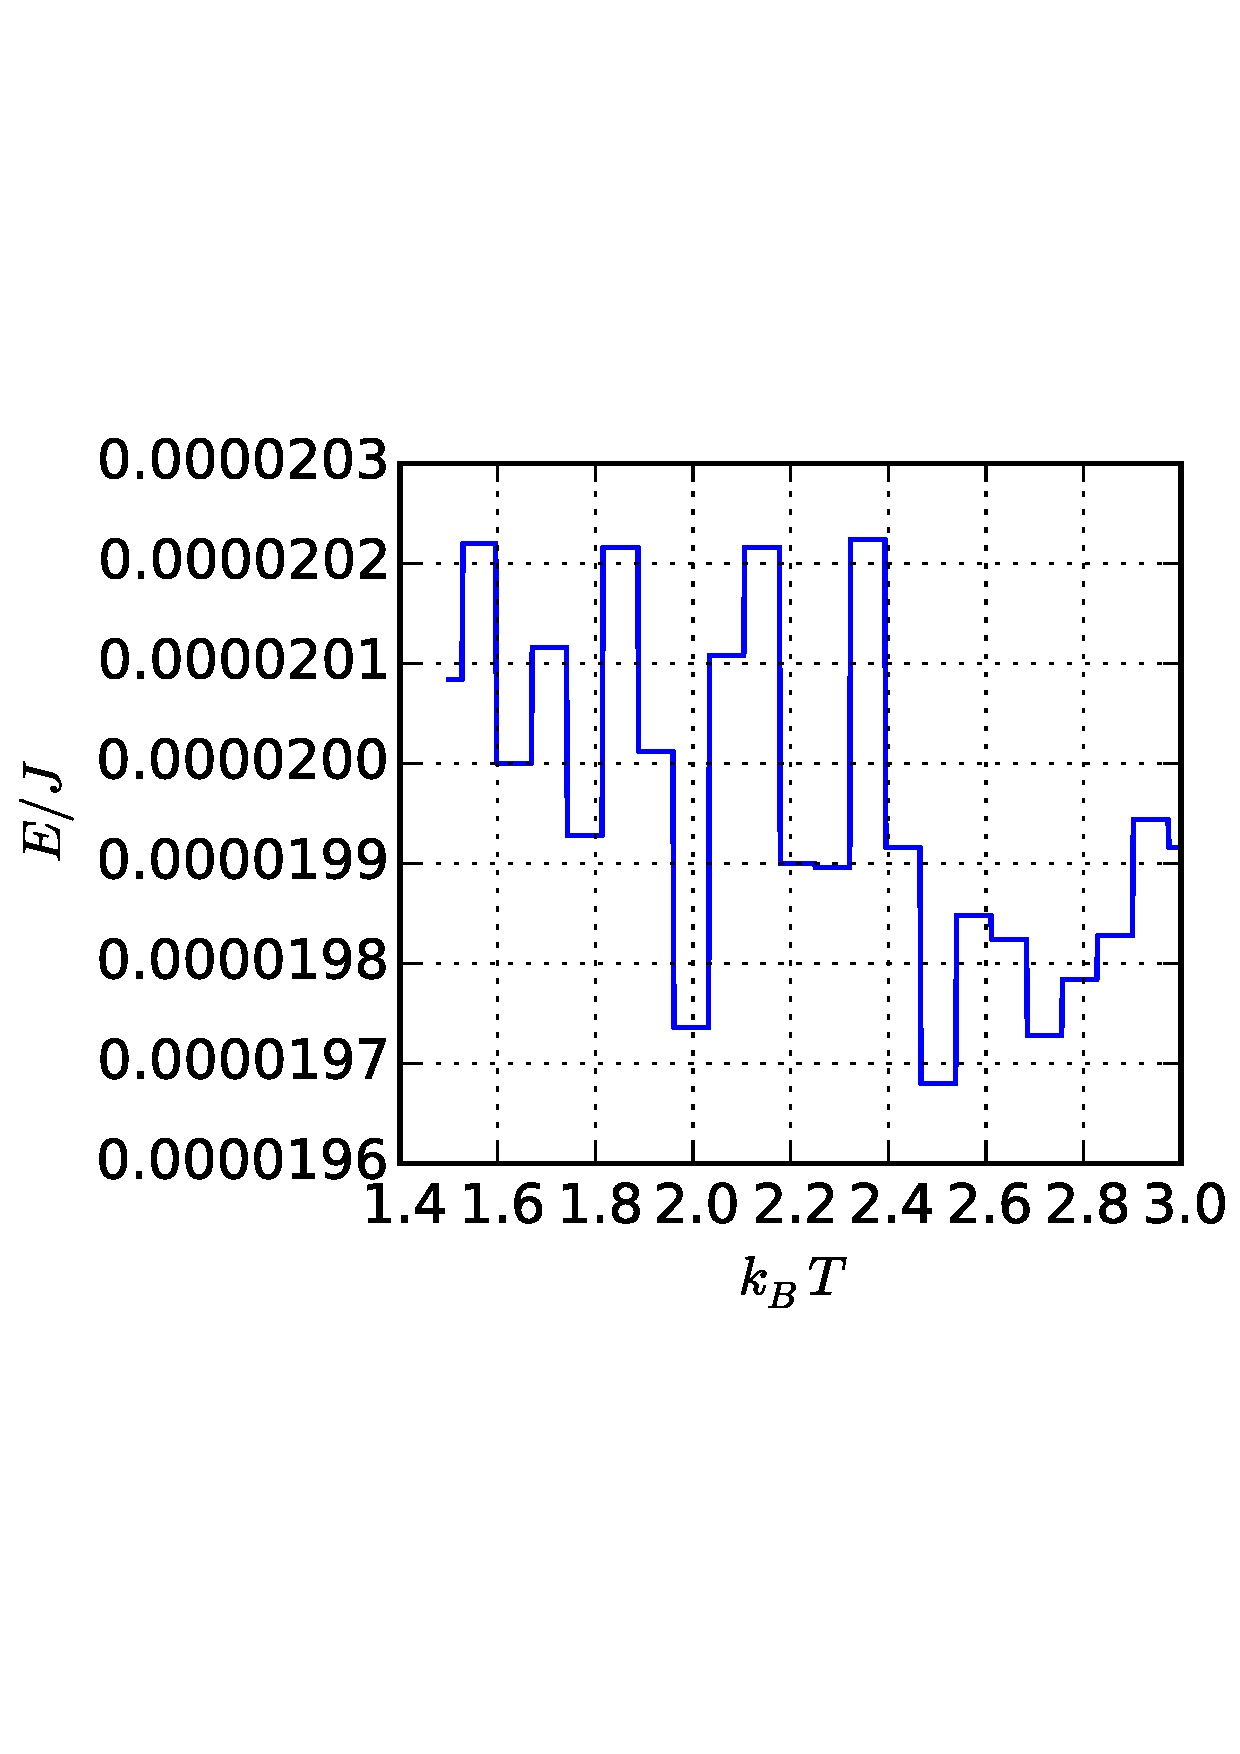
\includegraphics[width=0.8\linewidth]{new_york_skyline.pdf}
    \caption*{A Metropolis skyline as a function of temperature for 100000 MC-cycles.}

    \label{fig:new_york_skyline}
  \end{figure}
  \clearpage
  
  \begin{abstract}
    In this project we look at the Ising model in two dimensions. There are a
    set of physical quantities related to magnetic systems that are interesting
    to examine. We implement the Metropolis algorithm and compute various
    expectation-values for these quantities. For a $2\times2$ Ising model we
    derive the analytical expressions for these values and compare them with
    the numerically computed ones. We also examine what happen when we reach
    the thermodynamical limit, as the lattice size of the model increases.
    \noindent
    All source code can be found on my GitHub page: \\

    \centering{\href{https://github.com/qTipTip/FYS3150}{\githublogo \, \color{gray!50}\textit{github.com/qTipTip}}}
  \end{abstract}
  \tableofcontents
  % Explain the physical system we want to model
  % Introduce the Ising Model
  \section{The Ising model}

We first start by discussing the Ising Model in its most general form. We later
specialize the model to our specific needs.

\subsection{The general Ising model}
The \emph{Ising Model} is a model in statistical physics that describe phase
transitions in ferromagnetism\footnote{Ferromagnetism is the basic mechanism by
which certain materials form permanent magnets, or are attracted to magnets.
Ferromagnetism is the strongest type of magnetism.}. In this model we represent
magnetic dipole moments of atomic spins that can be in one of two states,
$\uparrow$ or $\downarrow$. The spins are arranged in a \emph{lattice}, which
enables us to relate one spin to its neighbors.

We first introduce some notation. Let $\Lambda$ be a set of lattice positions,
where each element in $\Lambda$ is assigned a set of neighboring sites. The
lattice then forms a graph. We assign for each $k \in \Lambda$ a variable
$\sigma_k$ which takes the value 1 or -1, representing the site's spin,
$\uparrow$ or $\downarrow$, respectively. We can now create a \emph{spin
configuration} $\sigma$ which is a specific configuration of this lattice.  For
two sites $i, j \in \Lambda$ one can talk about the \emph{interaction}
$J_{ij}$. Generally, for each $i \in \Lambda$ one also has an \textit{external
magnetic field} $h_i$ interacting with $i$.

We can talk of the \emph{energy} of a specific configuration, which is given by
the Hamiltonian
\begin{equation}
  \label{eq:general ising model}
  E = H(\sigma) = - \sum^{}_{\langle i k\rangle} J_{ij}\sigma_i\sigma_j - \mu \sum^{}_{j} h_j\sigma_j
\end{equation}
where the notation $\langle i j \rangle$ just means that we sum over adjacent
spins only.

In order to calculate relevant physical quantities for such a system, we need
an appropriate probability that describe the probability of finding the system
in a certain configuration. The \emph{configuration probability} is given by
the Boltzmann distribution
\begin{equation}
  \label{eq:configuration probability}
  P_\beta(\sigma) = \frac{e^{-\beta H(\sigma)}}{Z_\beta}
\end{equation}
where $Z_\beta$ is a normalization constant. We call $Z_\beta$ the
\emph{partition function} for the \emph{canonical ensemble}. It is interesting
to note that when increasing the temperature $T$, the probability
$P_\beta(\sigma)$ of finding the system in a specific configuration $\sigma$
\emph{decreases}. This is essentially due to the fact that when we increase the
temperature the probability of finding states in an unfavorable configuration
become probabilistically feasible in comparison with the most common
configurations.

When modeling a magnetic physical system there are certain physical quantities
that we are interested in. Firstly, the \emph{mean energy} given by
\begin{equation}
  \label{eq:mean energy}
  \langle E \rangle = \sum^{M}_{i=1} E_i P_\beta(\sigma) = \frac{1}{Z} \sum^{M}_{i=1} E_i e^{-\beta E_i}.
\end{equation}
The \emph{mean magnetization} is given by
\begin{equation}
  \label{eq:mean magnetization}
  \langle \mathcal{M} \rangle = \sum^{M}_{i=1} \mathcal{M}_i P_\beta(\sigma) =\frac{1}{Z} \sum^{M}_{i=1} \mathcal{M}_i e^{\beta E_i},
\end{equation}
where $\mathcal{M}_i = \sum^{}_{j \in \Lambda}\sigma_j$ for all configurations
$\sigma$ and $M$ denotes the number of possible configurations.  We are also
interested in the \emph{magnetic susceptibility} $\chi$ which tells us how much
an extensive parameter changes when an intensive parameter increases. It is
given by
\begin{equation}
  \label{eq:magnetic susceptibility}
  \chi = \frac{1}{k_BT}\left( \langle \mathcal{M}^2 \rangle - \langle \mathcal{M} \rangle^2 \right).
\end{equation}
The \emph{specific heat} $C_V$, which tells us how much the energy changes by
increasing the temperature, is given by
\begin{equation}
  \label{eq:specific heat}
  C_V = \frac{1}{k_BT^2} \left( \langle E^2 \rangle - \langle E \rangle ^2 \right).
\end{equation}

If we can make some assumptions about the interaction $J_{ij}$ we can classify
the Ising model.  If for all $i, j \in \Lambda$ we have
\begin{enumerate}[i)]
  \item $J_{ij} > 0$, we call the interaction \emph{ferromagnetic};
  \item $J_{ij} < 0$, we call the interaction \emph{antiferromagnetic};
  \item $J_{ij} = 0$, the spins are non-interacting.
\end{enumerate}

\subsection{Ising model specialized to our project}

We can make some simplifications to the general Ising model in order to tailor
it to our specific needs. First of all, we wish to examine the system with no
external magnetic field\footnote{This specific system was solved analytically
by Lars Onsager in 1944.}. We can therefore, due to $h_j = 0$ for all $j \in
\Lambda$, rewrite
\cref{eq:general ising model} as
\begin{equation}
  \label{eq:no magnetic ising}
  E = H(\sigma) = - \sum^{}_{\langle i k \rangle} J_{ij}\sigma_i\sigma_j.
\end{equation}
We also assume that the coupling constant $J_{ij}$ that describe the
interaction between neighboring spins as constant $J$ for all $i, j \in
\Lambda$. \Cref{eq:no magnetic ising} can then be read as
\begin{equation}
  \label{eq:constant interaction ising}
  E = H(\sigma) = - J\sum^{}_{\langle i k \rangle} \sigma_i\sigma_j
\end{equation}

In this project we wish to examine a ferromagnetic system, $J > 0$. This in
turn, means that it is favorable for neighboring spins to be parallel, as this
leads to a lower energy. This can be seen from the fact that $\sigma_i \sigma_j
= 1$ whenever spin $i$ and $j$ have the same sign.

\subsection{A $2\times2$ Ising model}
\label{sub:a_2times2_ising_model}

In order to get a feel for what these systems look like we examine a two
dimensional Ising model with lattice dimensions $L = 2$ and periodic boundary
conditions. Our model has $M = 2^4$ different configurations $\sigma$. The
energy for any arbitrary configuration is given by
\begin{align*}
  \label{eq:abitrary energy}
  E_i = -J \sum^{4}\nolimits_{\langle kl \rangle} \sigma_k\sigma_l.
\end{align*}

Based on this expression we see that whenever all spins are parallel we have a
configuration energy of $E_i = -8J$. In the cases where one single spin is
anti-parallel to the other three we have a configuration energy of $E_i = 0$.
If we have two parallel and two anti-parallel, the configuration energy is $E_i
= 0$ or $E_i = 8J$. Each energy state $E_i$ has a \emph{degeneracy}
$\Omega(E_i)$ which corresponds to the number of configurations with the same
energy state. The ground state for this system has degeneracy 2, so we can
either start with all spin up or all spin down and still be in the lowest
energy state possible. For a small $2\times2$ system such as this one, it is
not unlikely that we can transition from a configuration with all spin up to a
configuration with all spin down (although keeping the same energy level),
however this is unlikely for large lattices.

We are now interested in examining the physical quantities of interest
introduced above.  For the $2\times2$ Ising model these quantities have closed
form expressions. The work needed to show these relations are given in Appendix
A. The partition function for this particular system is given by
\begin{equation}
  \notag
  Z = \sum^{16}_{i=1} e^{-\beta E_i} = 4 \cosh (8\beta J) + 12.
\end{equation}
We can now compute the mean energy of the system. This gives
\begin{equation}
  \notag
  \langle E \rangle = 8J \frac{\sinh(8\beta J)}{\cosh (8\beta J)+3}
\end{equation}
Differentiating once more gives us an expression for the specific heat $C_V$
\begin{equation}
  \notag
  C_V = -\frac{64J^2 }{k_BT^2(\cosh(8\beta J) + 3)} \left( \cosh(8\beta J) - \frac{\sinh^2(8\beta J)}{\cosh(8\beta J)+3} \right)
\end{equation}
Similarly, we have a closed form expression for the susceptibility:
\begin{equation}
  \notag
  \chi = \frac{8 \left( e^{8\beta J} + 1 \right)}{\cosh(8\beta J) + 3} \frac{1}{k_BT}.
\end{equation}
We will later refer back to these specific values for the $2\times2$ Ising
model when we compare the analytical results to the numerically computed
values.
 
  % - 1D model
  % - 2D model
  %     - Square lattice Ising Model
  %       - interacting vs noninteracting
  %       - with our without external magnetic field
  %       - we wish to lower energy, explain parallel vs anti-parallel spin
  % Introduce the Metropolis Algorithm and why we want to use it
  \section{The Metropolis-Hastings Algorithm}

In this project we need random samples from a probability distribution
$P_\beta(\sigma)$ associated with the physical system we wish to model.
However, direct sampling can be difficult due to the fact that we need to
compute the partition function in order to express the probability distribution
in its entirety.

The Metropolis-Hastings algorithm is very well suited for this type of problem
because in order to sample from a specific distribution $P_\beta(\sigma)$ all
we need is a function $f$ proportional to the distribution density.

\subsection{The Metropolis Algorithm}
\label{sub:the_metropolis_algorithm}

Under the assumption that the proposed probability distribution function is
symmetric, we can make some simplifications to the Metropolis-Hastings
algorithm. This is what we call the Metropolis Algorithm.  The general
procedure can be described as follows:

\begin{enumerate}
  \item Initialization: We pick an initial sample.
  \item For every iteration: \\
    \begin{enumerate}
      \item We generate a new candidate for the new sample by picking a random element in the sample. 
      \item We calculate the acceptance ratio, which decides whether to reject
        or accept the new candidate. (This is why the Metropolis algorithm is
        good for this sort of problem. When computing the acceptance ratio, we
        divide out the normalization factor $Z$, which is the computationally
        heavy bit.)
      \item If the acceptance ratio is greater than one, we automatically
        accept the candidate. Otherwise, we accept the candidate with a
        probability equal to the acceptance ratio. In the case of a rejection
        the new sample is set to the previous one.
    \end{enumerate} 
\end{enumerate}

  % implementation
  \section{Implementation}
\label{sec:implementation}

In this section we take a closer look at some of the implementation specific
details in this project. The Ising model was implemented in \textsc{C++} and
the class \texttt{Ising.cpp} contains all the methods needed for simulating the
model.

\subsection{The Ising class}
\label{sub:the_ising_class}
I chose an object-oriented approach to this implementation because I wanted the
possibility of having class instances that represented a physical system at any
given time. By wrapping all the methods in a class I could easily rerun a
similar simulation for a different temperature by re-initializing the system
and keeping any values from the previous temperature.\footnote{If I managed to
pull any of this through by any stretch of the imagination can be discussed.} I
also had a boolean flag for checking whether the system had been previously
thermalized for a previous temperature - in that case, one could skip the
thermalization.

I did not manage to figure out a way of outputting data that would satisfy the
demands of all the text-problems in the project at once, so I did have to do
some monkey-patching for some of them.

The computationally heavy methods are the \texttt{simulate} and
\texttt{metropolis}-methods, where \texttt{simulate} calls \texttt{metropolis}
once for each Monte-Carlo cycle. If we let $L$ denote the grid dimension and
$M$ the number of Monte-Carlo cycles, then each call of the \texttt{metropolis}
method constitutes a complexity of $\mathcal{O}(L^2)$. The \texttt{simulate}
method calls \texttt{metropolis} $M$ times, hence the total complexity for one
simulation for one temperature is $\mathcal{O}(ML^2)$.

\subsection{Main method}
\label{sub:main_method}
The main method is fairly simple, given a temperature range $[T_1, T_2]$ it
assigns a subinterval based on the number of nodes running in parallel to each
node. Each node then proceeds to simulate the system for its assigned
temperature range, and outputs its data the same data-file. The sorting of the
data is done by \texttt{Python}. The parallelization is done using OpenMPI.

\subsection{Errors}
\label{sub:errors}

My program gives correct values for certain systems, and very wonky values for
other systems. I have not been able to determine whether this is an artifact of
running too few simulations, whether my temperature resolution should have been
higher, or whether it is an artifact introduced by the stochastic nature of the
algorithms or (most probable) there is a bug somewhere in my program.

Based on the plots produced, all the weird behavior occurs in the quantities
directly dependent on the magnetization, which might indicate that that is
where the problem lies.

  % simulations
  \section{Simulations}
\label{sec:simulations}
In this section we simulate the Ising model with various properties and examine
the properties of interest as functions of temperature $T$ and as functions of
lattice dimension $L$.
\subsection{$2\times2$ Ising with $T = 1$}
\label{sub:_2x2_ising_with_t_1_}
We assume we have a grid size of $2\times2$ as in
\cref{sub:a_2times2_ising_model}. We wish to consider these for a fixed
temperature $T' = 1.0$ in units of $Tk_B / J$.  We can therefore make the
following algebraic manipulations: Let $E'$ be the energy scaled by the
coupling constant $J$, that is $E' = E / J$. Similarly let $C_V' = C_V / k$ and
$\chi' = \chi J$. Let $N$ denote the number of Monte-Carlo cycles.

We can now easily compute the quantities using the closed form solutions given
in \cref{sub:a_2times2_ising_model}. The results are given in Table
\ref{tab:numerical comparison to analytical 2x2}. If we look at the error in
the numerical approximation, by means of the ratio between numerical and
analytical results we should expect a convergence towards 1. However, for the
specific heat, this is not the case, as the numerical results converge fairly
slowly. In \cref{fig:relative_error_1} we see that the magnetization and energy
converge quickly, after only two thousand cycles, the susceptibility follows
suit after some 10000 cycles while the specific heat never seem to converge,
even after a million cycles.
\begin{table}
  \centering
  \caption{Comparing numerical results to closed form analytical solutions for a $2\times2$ Ising model.}
  \label{tab:numerical comparison to analytical 2x2}
  \begin{tabular}{lcccc}
    \hline
    $N$ & $\langle E \rangle$ & $\langle \mathcal{M} \rangle$ & $C_V$ & $\chi$\\
    \hline
    100 & -2& 1 & 0& 0\\
    1000 & -2& 1& 0& 0 \\
    10000 & -1.9964& 0.67935& 0.0287482& 2.14783 \\
    100000 & -1.99654& 0.0276321& 0.0276321& 3.98085 \\
    1000000 & -1.99611& 0.05832& 0.0310754& 3.97991 \\
    \hline
    Analytical & -1.99598 & 0 & 0.03208 & 3.99330
  \end{tabular}
\end{table}
\begin{figure}
  \centering
  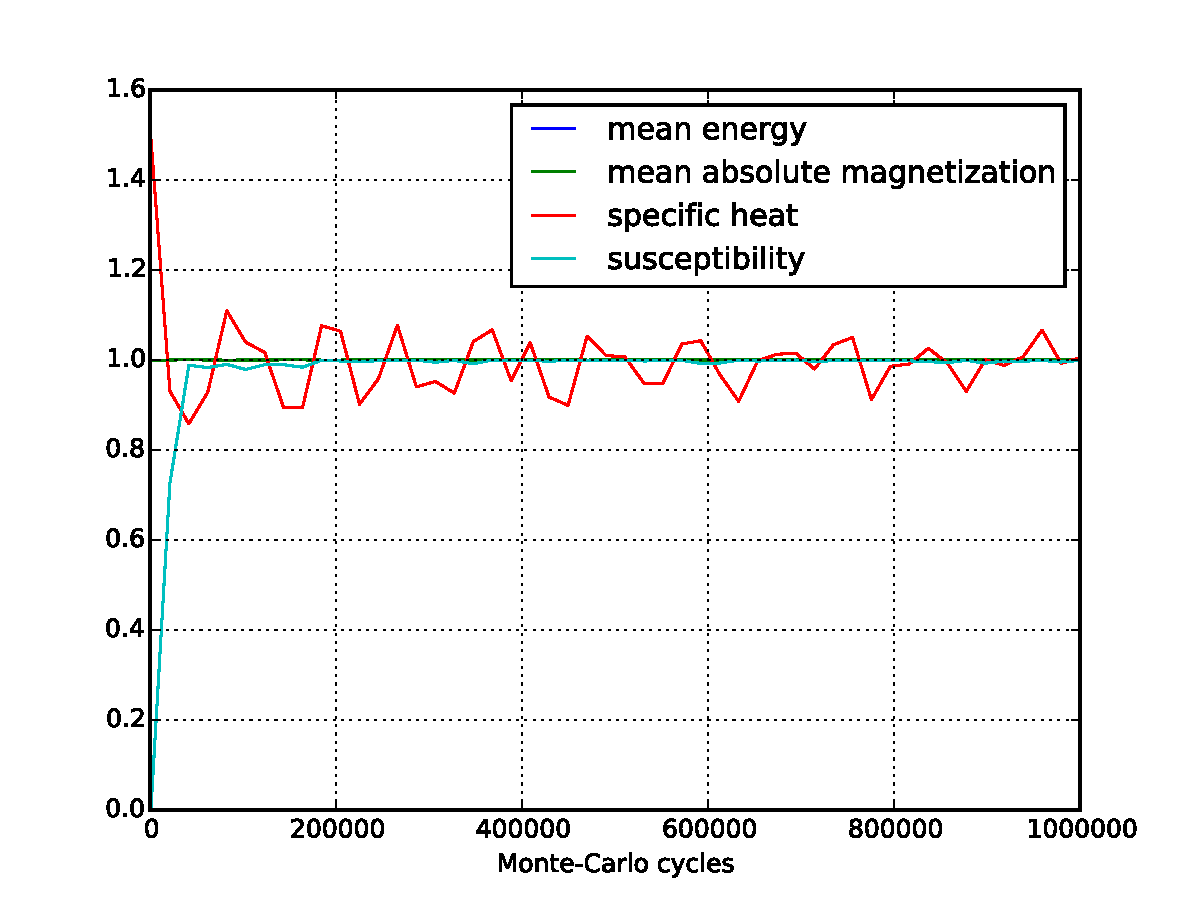
\includegraphics[width=0.8\linewidth]{task_b_million.pdf}
  \caption{This plot shows the convergence rate of the four quantities of
  interest. The magnetization and the energy converges after 2000 cycles, while
the susceptibility is slightly slower at 10000 cycles. The specific heat fails
to converge, even for a million cycles.}
  \label{fig:relative_error_1}
\end{figure}
\subsection{$20\times20$ Ising}
\label{sub:_20times20_ising}

We now consider a 20 by 20 lattice. We are interested in examining the number
of Monte-Carlo cycles needed to establish an equilibrium situation where it is
feasible to start calculating the expectation values. We start by plotting the
various expectation values as functions of the number of Monte-Carlo cycles.
We consider both an initial random configuration and an initial ordered
configuration for both the temperature $T = 1$ and $T = 2.4$.

While we're at it, we also keep track of the number of accepted configurations
and plot this as a function of temperature.
We see that for both random and ordered initial conditions, the system with a
temperature of $T = 1$ stabilizes fairly rapidly as can be seen in
\cref{fig:1_mc_ordered} and \cref{fig:1_mc_random} With a temperature of $T =
2.4$ however, the expectation values are a bit jittery at first, and seem to
somehow converge for upwards of 4000 cycles. This can be seen in
\cref{fig:2_mc_ordered} and \cref{fig:2_mc_random}.
\begin{figure}
  \centering
  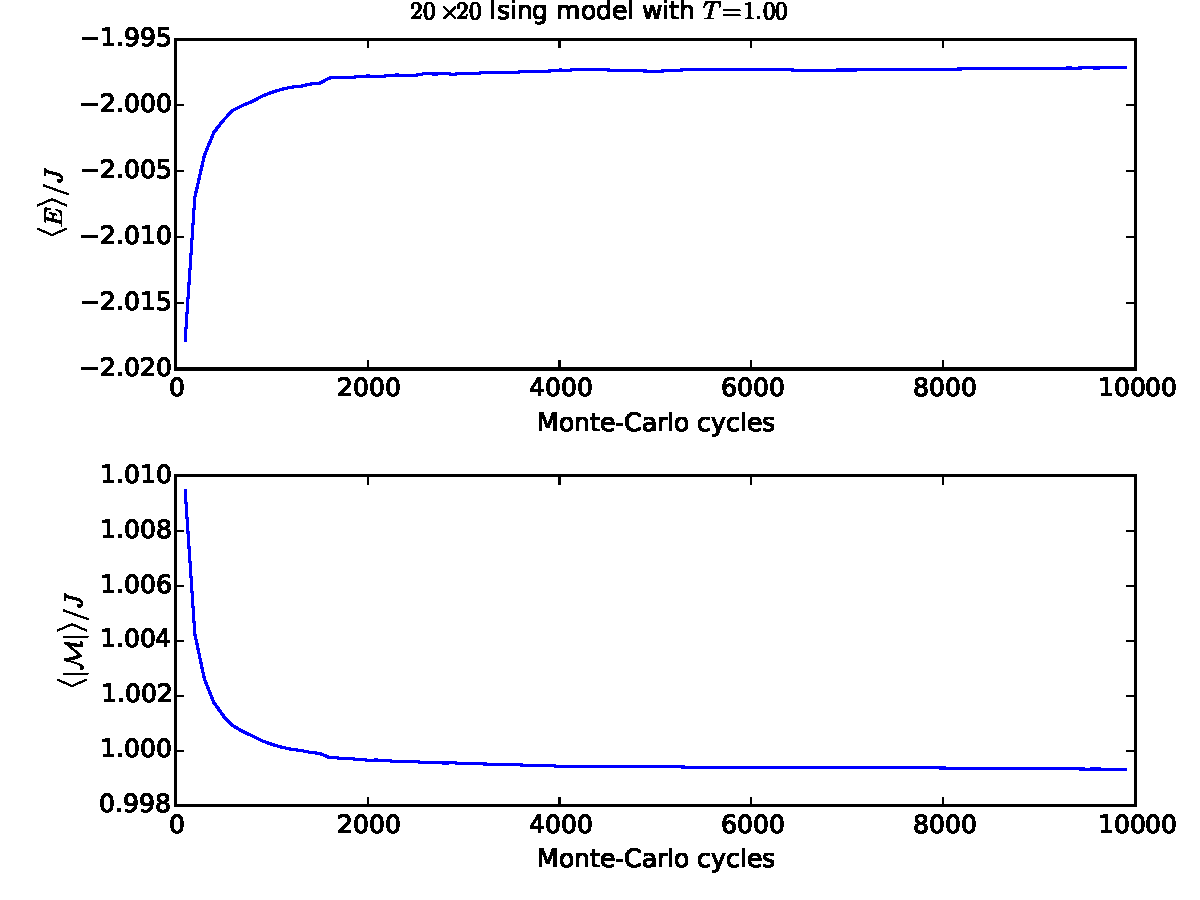
\includegraphics[width=0.8\linewidth]{1_mc_ordered.pdf}
  \caption{Plotting the expected energy and expected absolute magnetization as
  functions of the number of Monte-Carlo cycles. This system has a temperature
of $T = 1$ and an ordered initial configuration. In this situation the values
seem to stabilize around $2000$ cycles.}
  \label{fig:1_mc_ordered}
\end{figure}
\begin{figure}
  \centering
  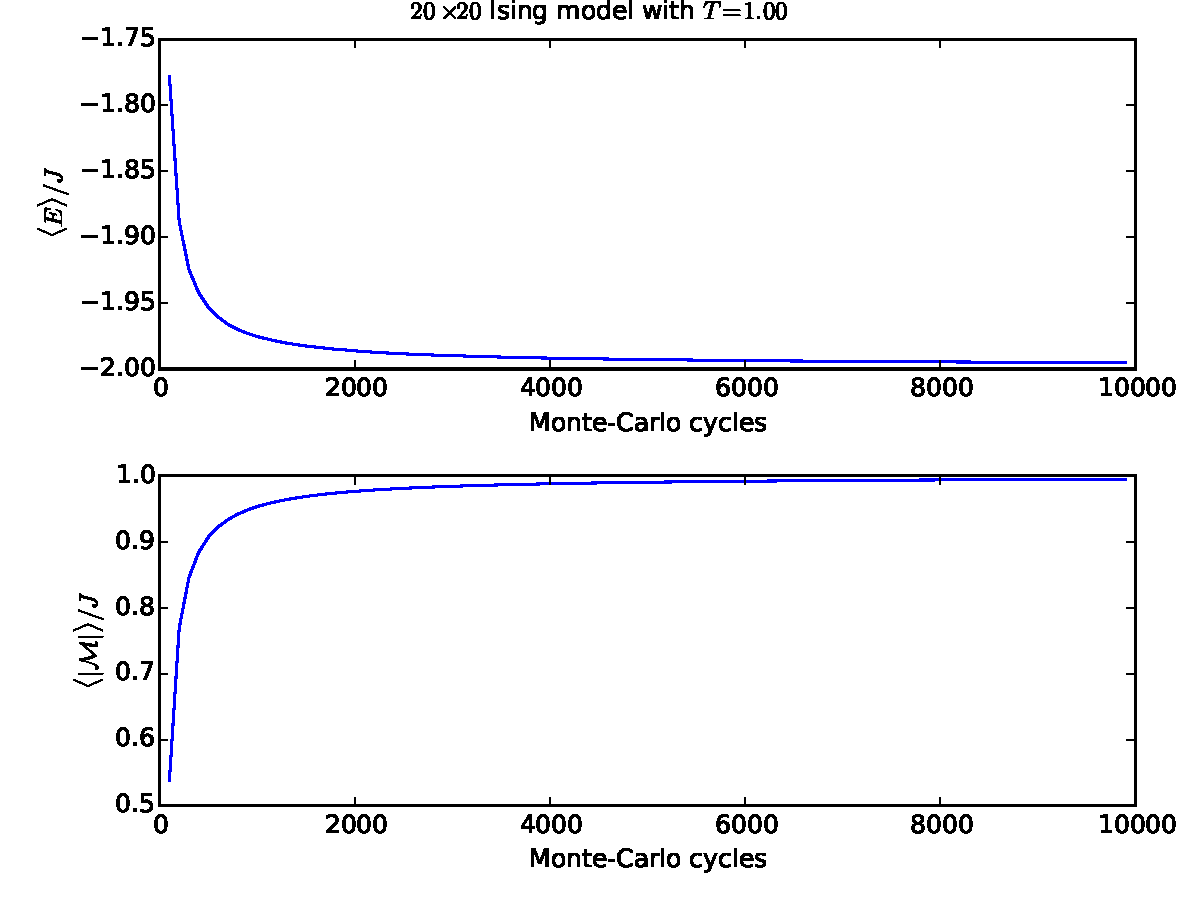
\includegraphics[width=0.8\linewidth]{1_mc_random.pdf}
  \caption{Plotting expected energy and expected absolute magnetization as
  functions of the numbers of the number of Monte-Carlo cycles. System has a
temperature of $T = 1$ with a random initial configuration. The system
stabilizes around $2000$ cycles.}
  \label{fig:1_mc_random}
\end{figure}

\begin{figure}
  \centering
  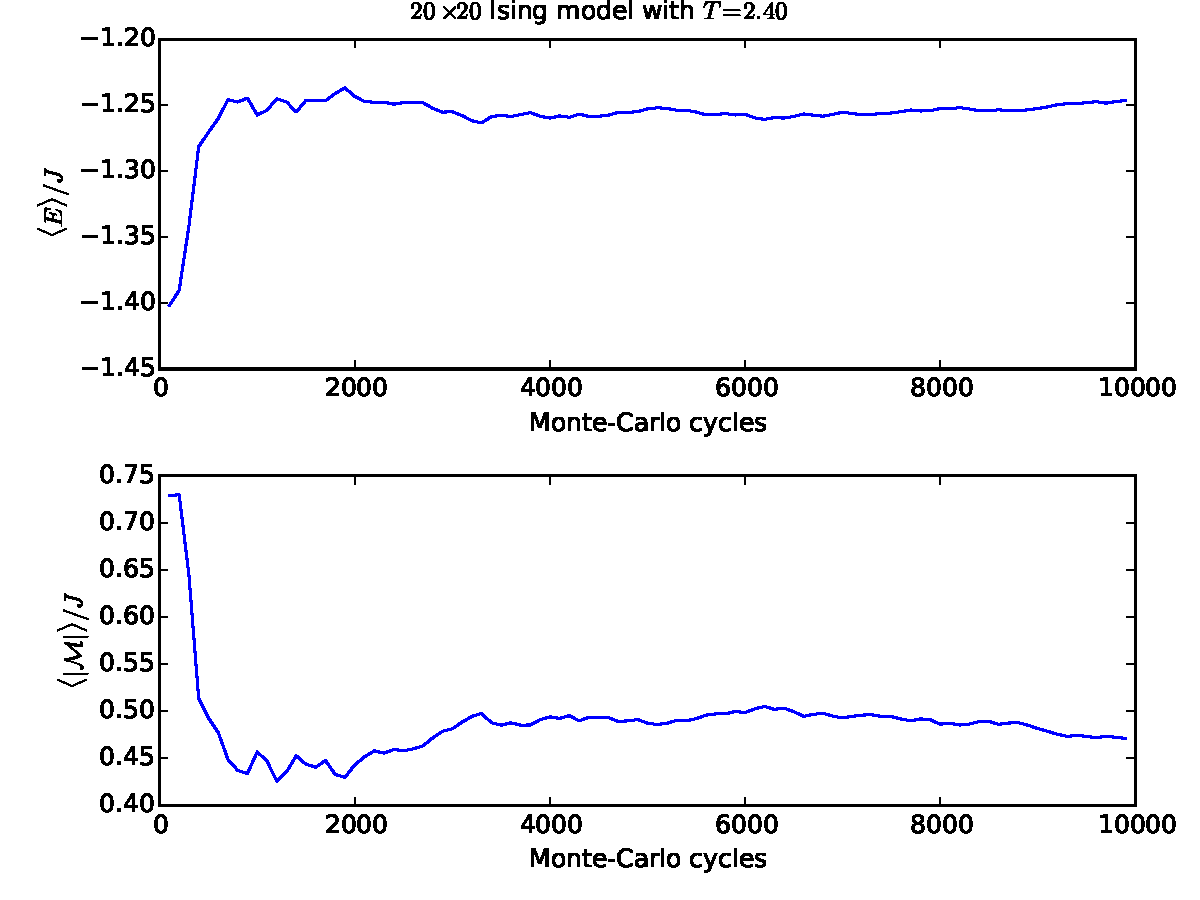
\includegraphics[width=0.8\linewidth]{2-4_mc_ordered.pdf}
  \caption{Plotting expected energy and expected absolute magnetization as
  functions of the numbers of the number of Monte-Carlo cycles. System has a
temperature of $T = 2.4$ with a random initial configuration. The system
stabilizes around $4000$ cycles.}
  \label{fig:2_mc_ordered}
\end{figure}

\begin{figure}
  \centering
  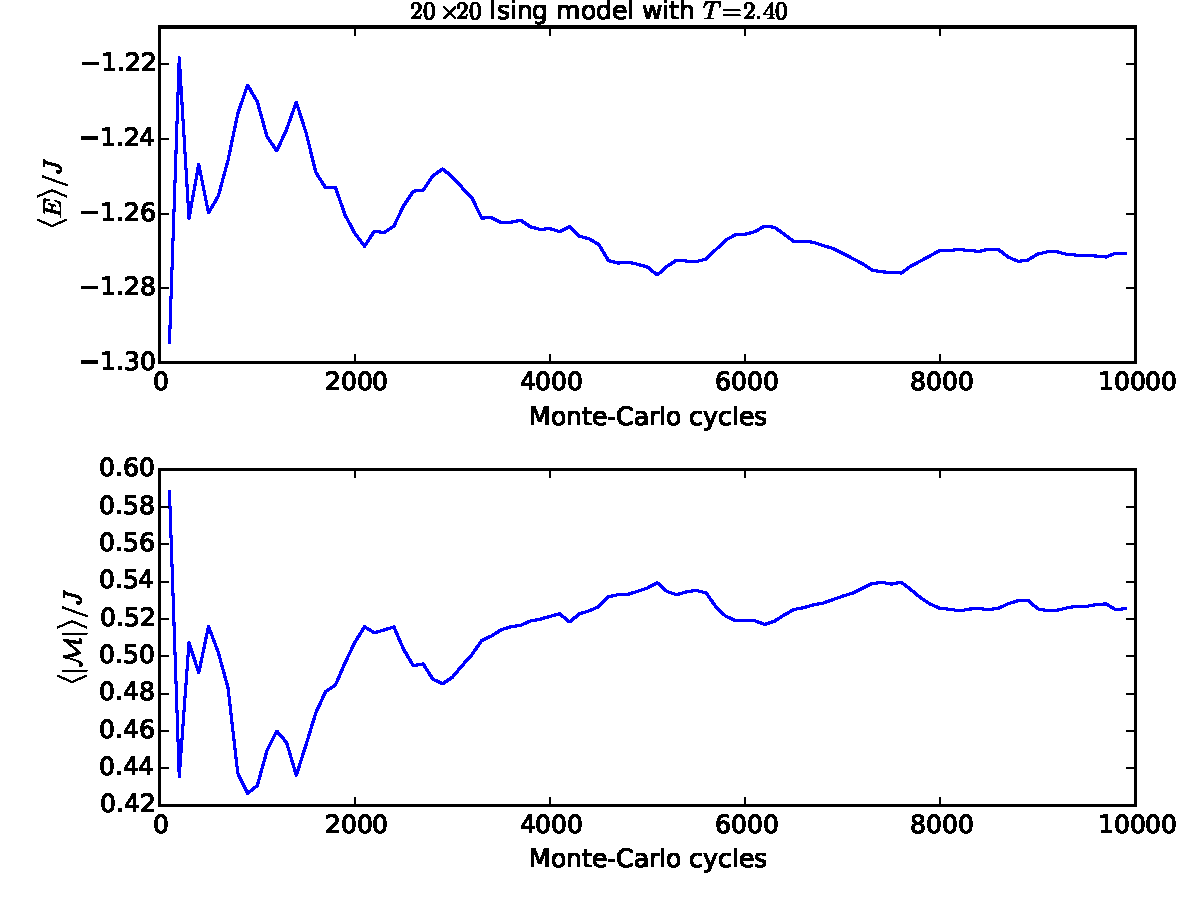
\includegraphics[width=0.8\linewidth]{2-4_mc_random.pdf}
  \caption{Plotting expected energy and expected absolute magnetization as
  functions of number of Monte-Carlo cycles. System has a temperature of $T =
2.4$ with a random initial configuration. The values seem to stabilize around
4000 cycles.}
  \label{fig:2_mc_random}
\end{figure}

When we consider the number of accepted states as a function of temperature, we
see that it increases drastically as the temperature increases. This is of
course in accordance with what we would assume if we were to just look at the
probability of any given state. As the temperature increases, the probability
of any arbitrary state becomes close to the probability of the most likely
state. You can view this as ''unlocking'' more possible states as the
temperature increases. The results are shown in \cref{fig:accepted_configs}.
\begin{figure}
  \centering
  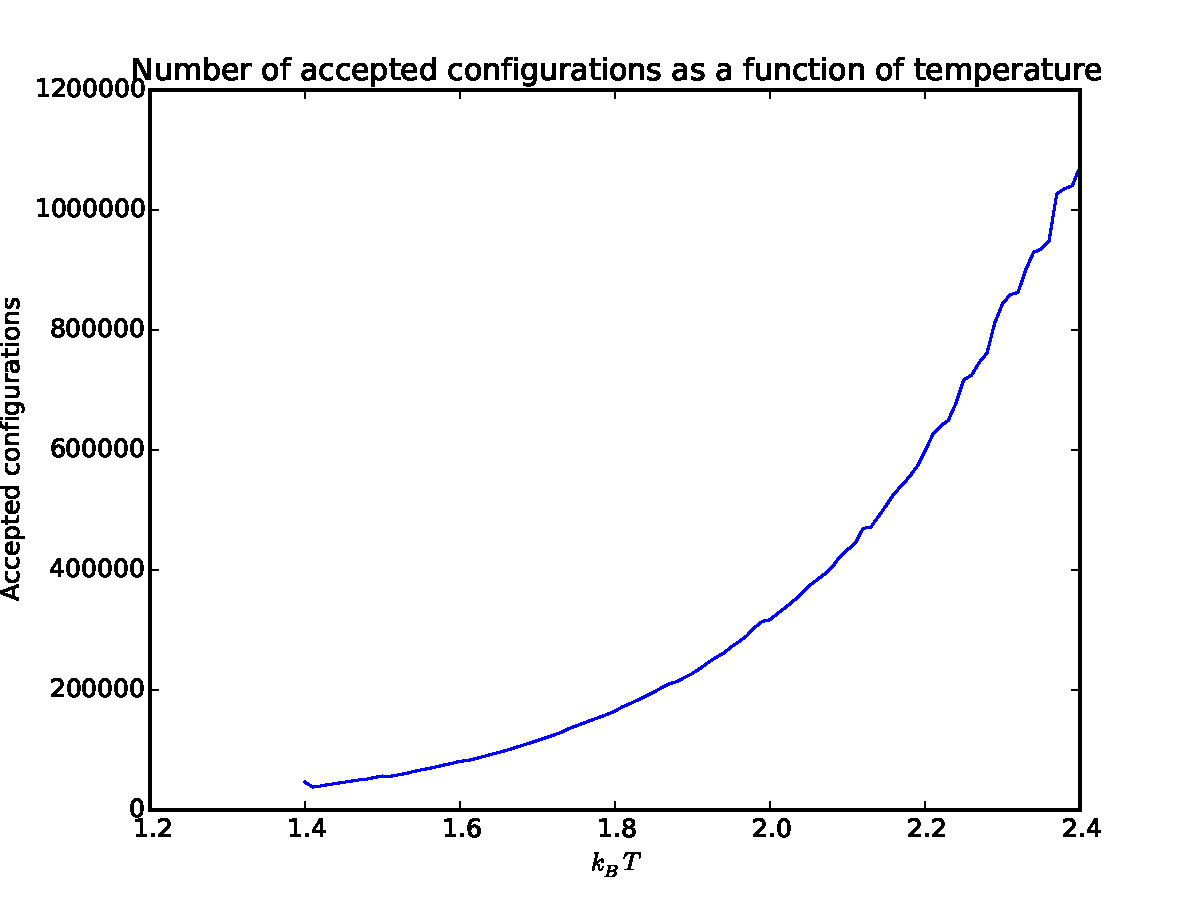
\includegraphics[width=0.8\linewidth]{accepted_configs.pdf}
  \caption{Number of accepted configurations as a function of temperature. The
  results are in accordance with the mathematical expression for the
probability of any given state. This number is probably more interesting when
divided by total number of configurations looked at. We then get a graph
converging to some number $t \in \left[ 0, 1 \right]$ which corresponds to the
probability of a configuration being accepted.}
  \label{fig:accepted_configs}
\end{figure}

We also want to look at the probability $P(E)$ for this same system for both
temperatures of $T=1$ and $T = 2.4$. These are given in \cref{fig:probability
1} and \cref{fig:probability 24}. If we compare these results to the computed
energy variance $\sigma_E^2$ which for $T = 1$ is evaluated to $\sigma_E^2
\approx 9.34 $ and for $T = 2.4$ is evaluated to $\sigma_E^2 \approx  3229$ we
see that the plots seem reasonable.\footnote{These are not per spin as the
other quantities discussed.}
For $T = 1$ the standard deviation $\sigma_E \approx 3.06$ and for $T = 2.4$ it
is $\sigma_E \approx 56.8$. The physical interpretation of this is that when
increasing the temperature we accept more possible states as previously
discussed. We therefore see more energy states appearing further from the most
likely state.
\begin{figure}
  \centering
  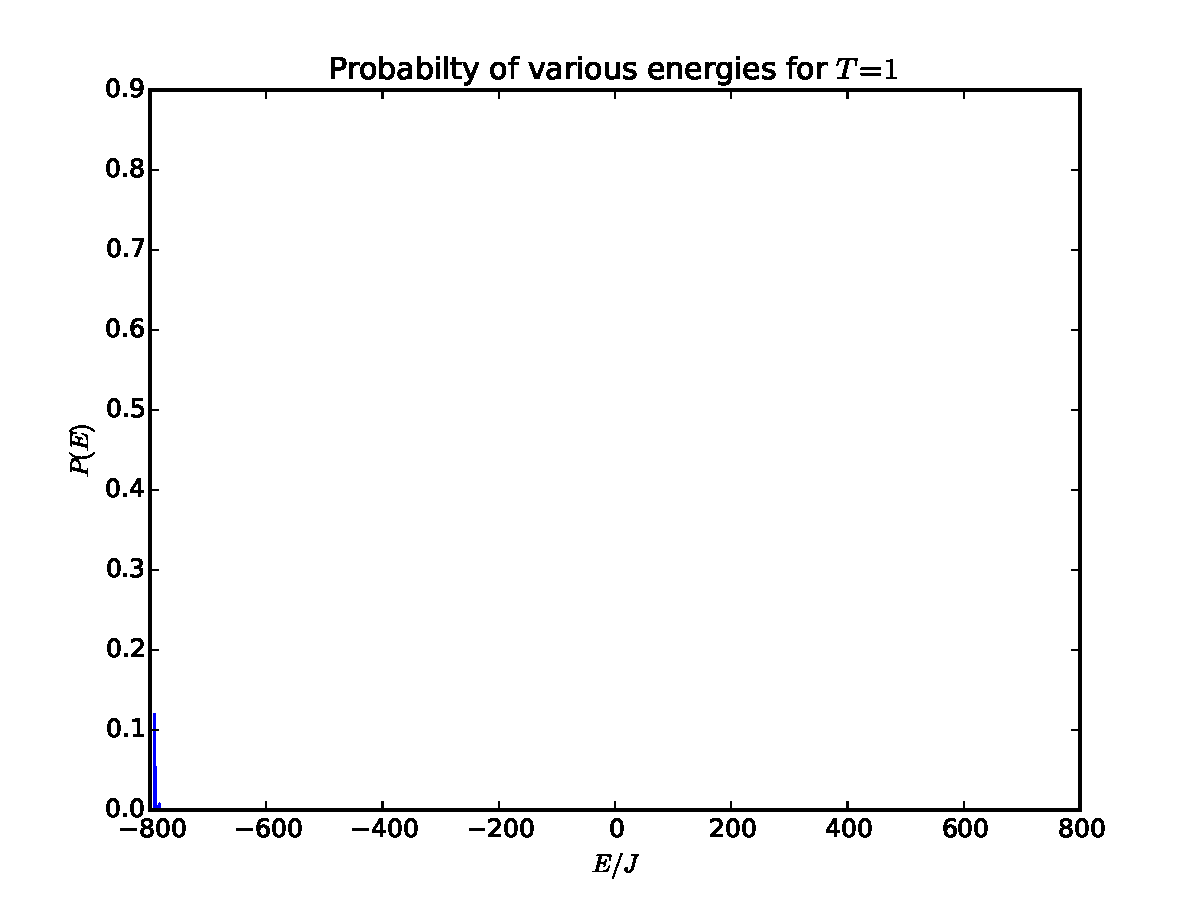
\includegraphics[width=0.8\linewidth]{probability_1.pdf}
  \caption{The probabilities of various energy levels in a Ising model with a
    temperature of $T = 1.0$. The energy states with a high probability are
    squashed all the way to the left which seems reasonable, since we start
    with an initially ordered configuration already in its ground state. Under
  low temperatures, the chance of escaping this ground state is very slim.}
  \label{fig:probability 1}
\end{figure}

\begin{figure}
  \centering
  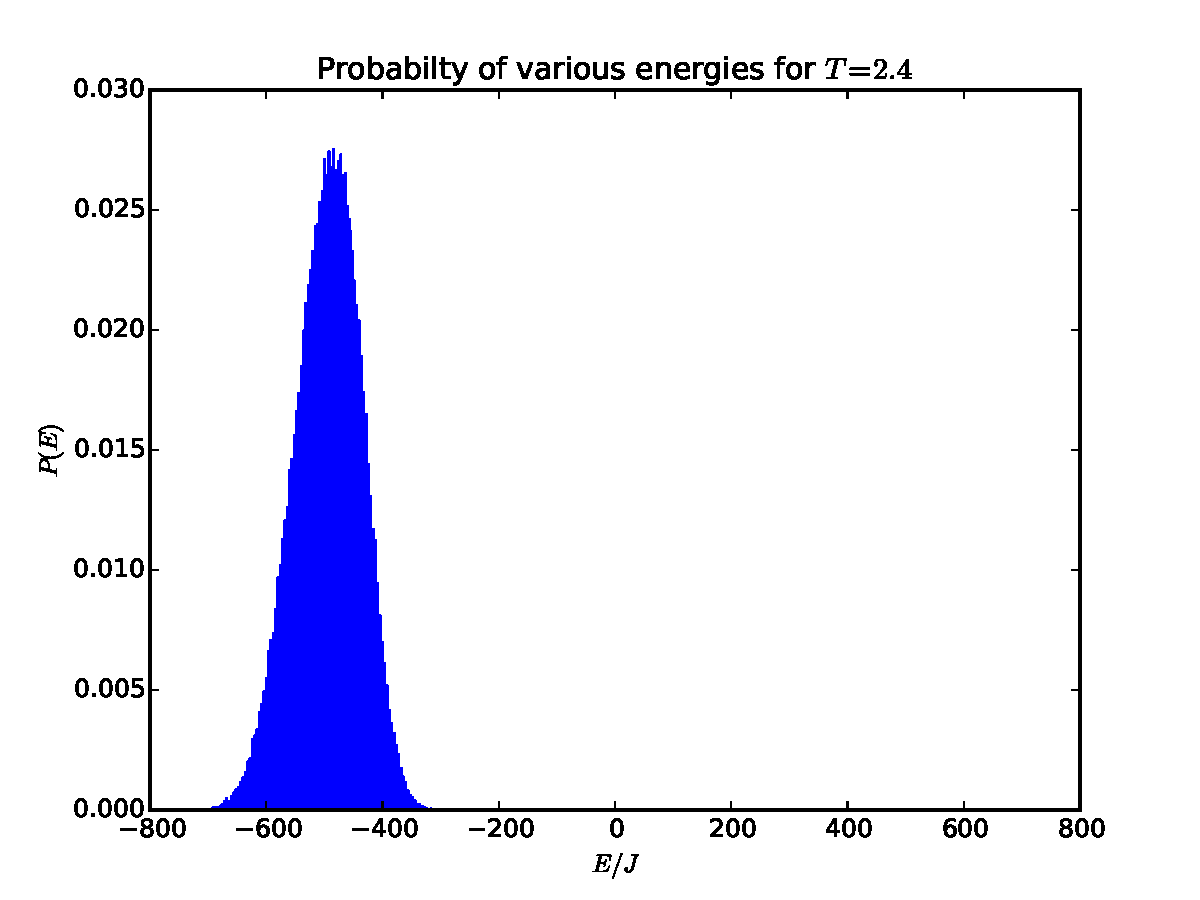
\includegraphics[width=0.8\linewidth]{probability_24.pdf}
  \caption{The probabilities of various energy levels in a Ising model with a
  temperature of $T = 2.4$. Here the energy states of interest are distributed
more evenly with the distribution centered at about $-500J$.}
  \label{fig:probability 24}
\end{figure}

\subsection{The critical temperature $T_C$ and the thermodynamical limit.}

In this section we examine the properties of the Ising model for various grid
sizes, and we fix our attention specifically to the temperature interval
$\left[ 2.0, 2.4 \right]$ as we know that the system undergoes a phase
transition for $T \approx 2.3$.

If we look at the plots given in \cref{fig:task_f_20}, \cref{fig:task_f_40},
\cref{fig:task_f_60} and \cref{fig:task_f_80} we see that increasing the grid
size changes the behavior of the system close to the critical temperature.
Firstly, we see that the susceptibility $\chi$ dramatically increase. As far as
I have understood, this means that near critical temperature, any change in
intensive parameters that does not depend on the number of particles in the
system constitutes a large change in magnetization. We also see that as the
absolute magnetization converges to zero for increasing grid size near critical
temperature which definitely indicates that the system is undergoing a phase
transition. I used python to visualize this phase transition for a
$200\times200$-model. A \texttt{GIF} can be found in the
\texttt{animations}-folder.

Near the critical temperature it turns out we can look at the behavior of certain physical quantities by means of a power law.
For $\beta = 1/8$, $\alpha = 0$ and $\gamma = 7/4$ we see that the mean magnetization, specific heat and susceptibility as functions of temperature $T$ closely follows the following relations:
\begin{align*}
  \langle \mathcal{M}(T) \rangle &\sim \left( T - T_C \right)^\beta \\
  C_V(T) &\sim \left| T_C - T \right|^\alpha \\
  \chi(T) &\sim \left|T_C - T\right|^\gamma
\end{align*}
We can also look at the relation between a quantity computed for a finite
lattice size and the corresponding quantity in the thermodynamical limit. We
now wish to see whether we can approximate the thermodynamical limit using our
simulations of finite grids. The critical temperature as a function of lattice
size satisfies the following relation:
\begin{equation}
  \notag
  T_C(L) - T_C(L = \infty) = aL^{-1/v},
\end{equation}
where for $v = 1$ the exact result for critical temperature is ${kT_C/J = 2 /
\ln(1+\sqrt{2})}$ which evaluates to approximately 2.269. Rearranging the equation gives us
\begin{equation}
  T_C(L = \infty) = T_C(L) - aL^{-1/v}.
\end{equation}

We can now look at our simulations and see if we can approximate the critical
temperature in the thermodynamical limit. My simulations are not sufficiently
good for me to be able to point out the differences in critical temperature for
the various grid sizes, so all I know is that it is located between $T=2.25$
and $T=2.30$. That being said, the only reasonable assumption based on the
results my simulations produced is that $T_C$ is 2.275 for all lattice sizes.
However, this renders us unable to calculate the factor $a$ in the following relations:
\begin{align*}
  T_C(L = \infty) &= T_C(20) - a20^{-1} = 2.275 - \frac{a}{20}\\
  T_C(L = \infty) &= T_C(40) - a40^{-1} = 2.275 - \frac{a}{40}\\
  T_C(L = \infty) &= T_C(60) - a60^{-1} = 2.275 - \frac{a}{60}\\
  T_C(L = \infty) &= T_C(80) - a80^{-1} = 2.275 - \frac{a}{80}
\end{align*}
\begin{figure}
  \centering
  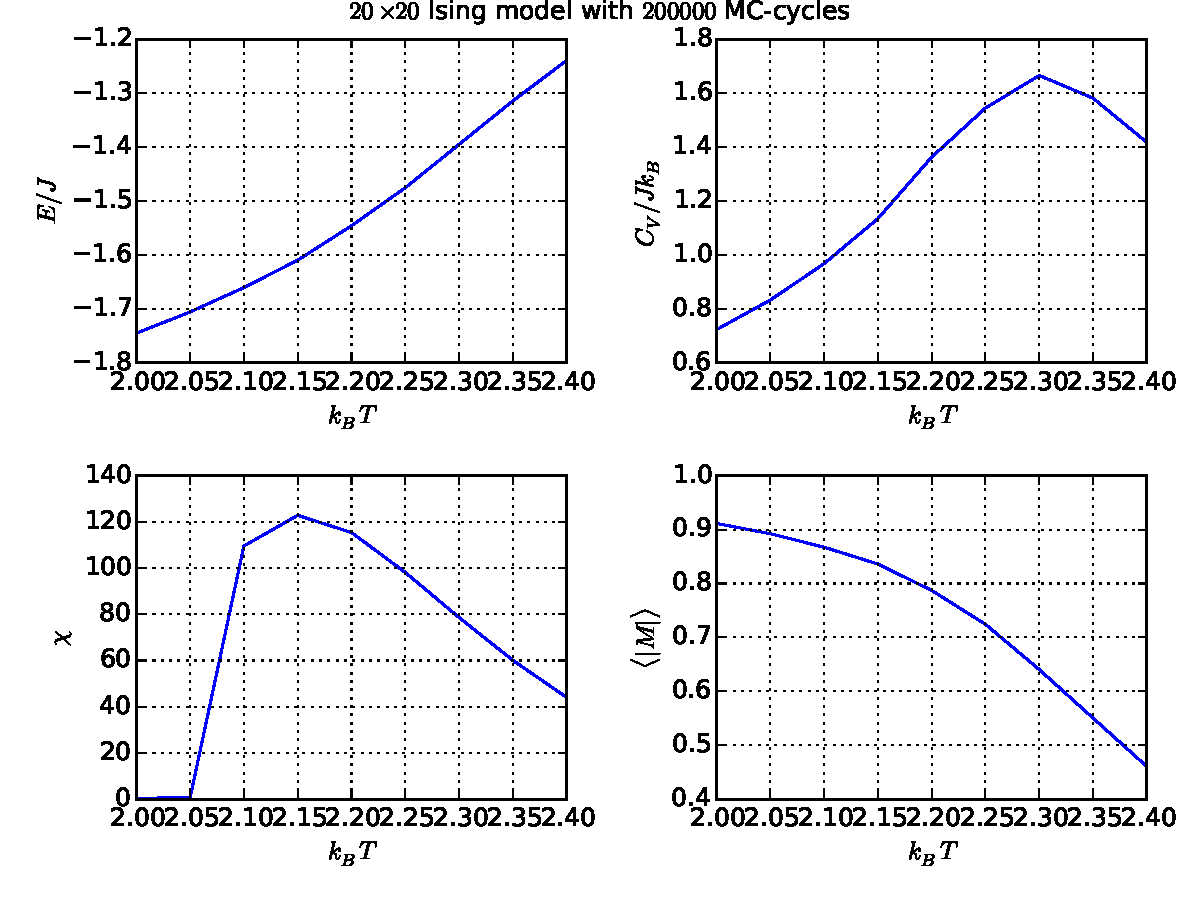
\includegraphics[width=0.8\linewidth]{task_f_20.pdf}
  \caption{Physical quantities near the critical temperature $T_C$ for a grid size of 20.}
  \label{fig:task_f_20}
\end{figure}

\begin{figure}
  \centering
  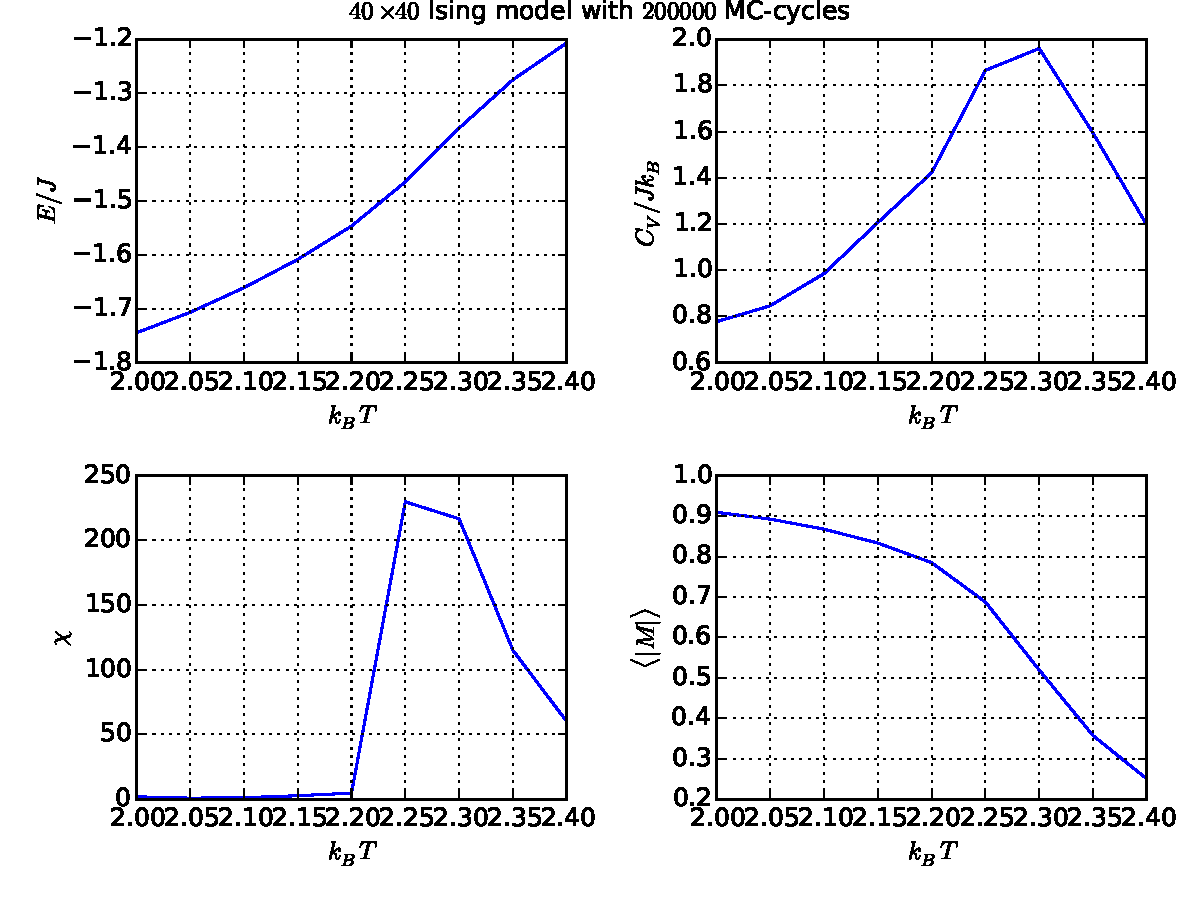
\includegraphics[width=0.8\linewidth]{task_f_40.pdf}
  \caption{Physical quantities near the critical temperature $T_C$ for a grid size of 40.}
  \label{fig:task_f_40}
\end{figure}

\begin{figure}
  \centering
  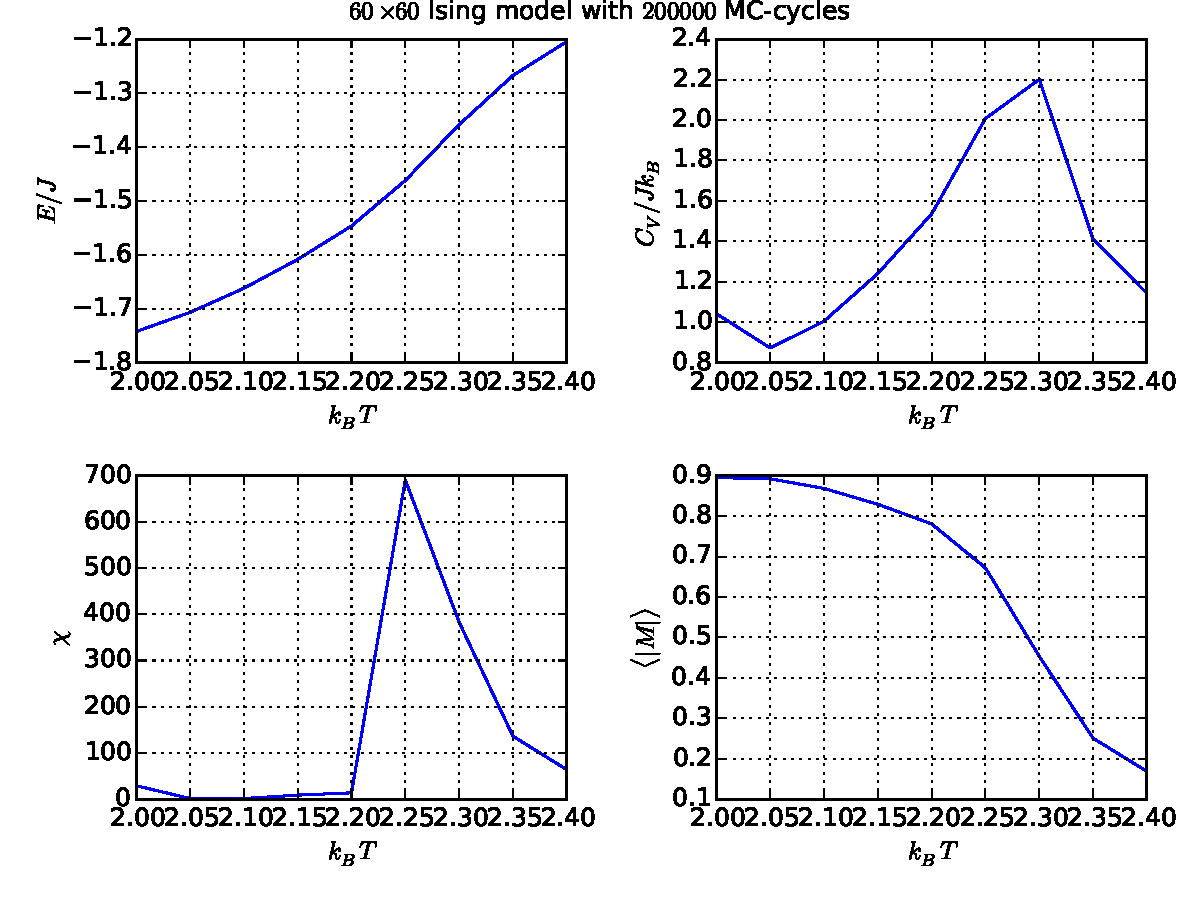
\includegraphics[width=0.8\linewidth]{task_f_60.pdf}
  \caption{Physical quantities near the critical temperature $T_C$ for a grid size of 60.}
  \label{fig:task_f_60}
\end{figure}

\begin{figure}
  \centering
  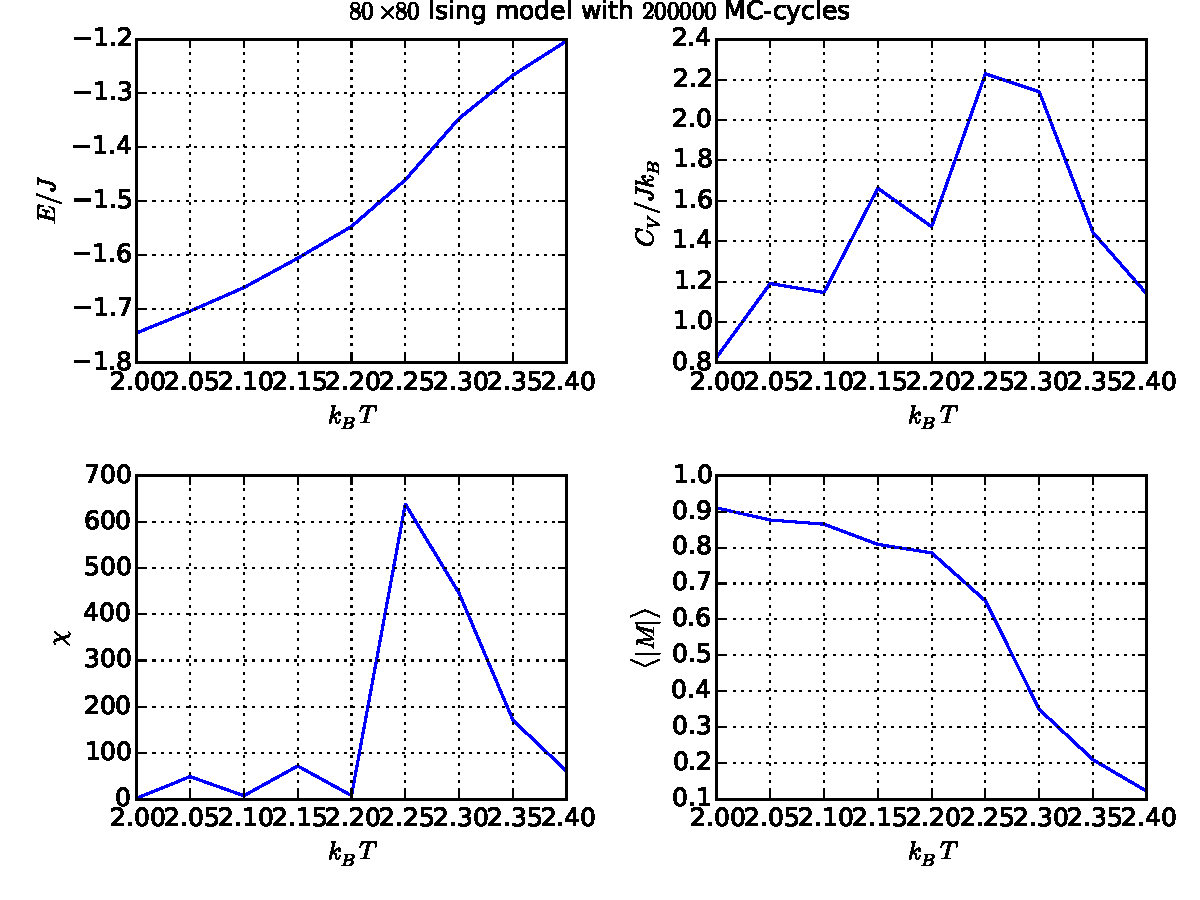
\includegraphics[width=0.8\linewidth]{task_f_80.pdf}
  \caption{Physical quantities near the critical temperature $T_C$ for a grid size of 80.}
  \label{fig:task_f_80}
\end{figure}

  % Calculations of 2x2 analytical quantities
  \clearpage
  \section{Conclusion}
\label{sec:conclusion}

In this project we implemented the Metropolis algorithm in an effort of
simulating the Ising model for varying sizes of finite lattices. My simulations
gave me accurate results for certain models and results that did not converge
properly for others. This is extra apparent in the plots for varying grid sizes
when looking for the critical temperature. Despite these issues I feel that I
was able to answer most the questions asked in the problem text.

  \appendix
  \section{Analytical derivations}
\label{sec:analytical_derivations}

In this section we derive the closed form analytical expressions for the
physical quantities for a $2\times2$ Ising model. The mean energy and specific
heat of a thermodynamical system can be expressed in terms of the partition
function.
\begin{align*}
  \langle E \rangle = - \frac{\partial}{\partial \beta} \ln Z; &&  \langle C_V \rangle = \frac{1}{kT^2}\frac{\partial^2}{\partial\beta^2}\ln Z.
\end{align*}
We recall that the partition function for a $2\times2$ model is given by ${Z = 4\cosh(8\beta J) + 12}$. The mean energy then becomes
\begin{align*}
  \langle E \rangle = -\frac{\partial}{\partial\beta} \ln \left( 4\cosh(8\beta J) + 12 \right) = -8J\frac{\sinh(8\beta J)}{\cosh(8\beta J+3)}, 
\end{align*} 
and the mean specific heat becomes
\begin{align*}
  \langle C_V \rangle  &= -\frac{1}{kT^2}\frac{\partial}{\partial\beta}\left(-8J\frac{\sinh(8\beta J)}{\cosh(8\beta J+3)}\right)\\
                       &= \frac{1}{kT^2}\frac{64J^2}{\cosh(8\beta J)+3} \left( \cosh(8\beta J) - \frac{\sinh^2(8\beta J)}{\cosh(8\beta J)+3} \right).
\end{align*}

The magnetization of a configuration is given by the sum of all spins. In order
to examine the mean magnetization of a system of a given lattice size, we
simply sum over all possible magnetizations multiplied by the probability of
the system being in each such configuration. Mathematically, this translates into
\begin{equation}
  \notag
  \langle \mathcal{M} \rangle = \frac{1}{Z} \sum^{M}_{i=1} M_i e^{-\beta E_i}.
\end{equation}
For a simple $2\times2$ lattice this simply reduces to counting all the
possibilities and this gives us that the mean magnetization is
\begin{equation}
  \notag
  \langle \mathcal{M} \rangle = \frac{1}{Z} \left( -4e^{8\beta J} - 8e^0 + 8e^0 + 4e^{8\beta J} \right) = 0.
\end{equation}
If we were to consider the mean of the absolute magnetization $|\mathcal{M}|$, then this simply becomes
\begin{equation}
  \notag
  \langle |\mathcal{M}| \rangle = \frac{1}{Z} \left( 4e^{8\beta J} + 8e^0 + 8e^0 + 4e^{8\beta J} \right) = \frac{4 + 2e^{8\beta J}}{\cosh(8\beta J)+3}.
\end{equation}

The susceptibility $\chi$ of a thermodynamical system can be calculated if we
know the variance $\sigma_\mathcal{M}^2$ of the magnetization and is given by 
\begin{equation}
  \notag
  \chi = \frac{1}{kT}\sigma_\mathcal{M}^2.
\end{equation}
We first start by computing the variance of the magnetization:
\begin{align*}
  \sigma_\mathcal{M}^2 = \langle \mathcal{M}^2 \rangle - \langle \mathcal{M} \rangle^2 = \frac{32}{Z}\left( e^{8\beta J} + 1 \right) - 0 = \frac{8 \left( e^{8\beta J} + 1 \right)}{\cosh(8\beta J) + 3}.
\end{align*}
The susceptibility then reads
\begin{equation}
  \notag
  \chi = \frac{8 \left( e^{8\beta J} + 1 \right)}{kT(\cosh(8\beta J) + 3)}.
\end{equation}

\end{document}
